\section{Models}

\begin{frame}{Overview}
	\begin{itemize}
		\item gnee
	\end{itemize}
\end{frame}

%%%%%%%%%%%%%%%%%%%%%%%%%%%%%%%%%%%%%%%%%%%%%%%%%%%%%%%%%%%%%%%%%%%%%%%%%
\subsection{Concatenation Approaches}

\begin{frame}{Concatenation Approaches}
Concatenation approaches to DLNMT consist in feeding a standard encoder-decoder architecture with a concatenation of sentences. 
	\begin{figure}
		\centering
		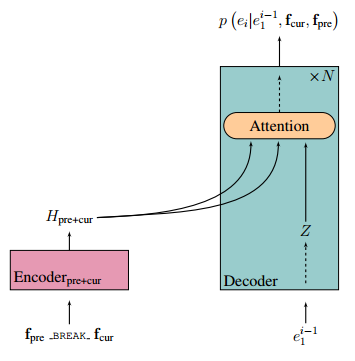
\includegraphics[width=0.45\linewidth]{Images/concatenation}
		\label{fig:concatenation}
	\end{figure}
\end{frame}

\begin{frame}{Concatenation Approaches}
For instance:
	\begin{itemize}
		\item \cite{tiedemann_neural_2017} firstly introduced this approach proposing an RNN-based model that incorporate the preceding sentence by prepending it to the current one, separated by a $<$CONCAT$>$ token. They propose two methods:
			\begin{itemize}
				\item \textbf{2-TO-2}: the previous and the current sentences are translated together. The translation of the current sentence is then obtained by only retaining the tokens following the concatenation token.
				\item \textbf{2-TO-1}: only the current sentence is translated. 
			\end{itemize}
		\item \cite{agrawal_contextual_2018,scherrer_analysing_2019} investigated the concatenation approach with the Transformer as base model, extending the number of context sentences both on the source (s:-3,+1) and the target (t:-2) side.
	\end{itemize}
\end{frame}

%%%%%%%%%%%%%%%%%%%%%%%%%%%%%%%%%%%%%%%%%%%%%%%%%%%%%%%%%%%%%%%%%%%%%%%%%
\subsection{Separate Encoding Approaches}

\begin{frame}{Separate Encoding Approaches}
Separate encoding approaches to DLNMT consist in encoder-decoder models that encode the current and context sentences separately. This can be undertaken by:
	\begin{itemize}
		\item \textbf{Multiple encoders} working in parallel for the current and previous sentence. E.g. \cite{wang_exploiting_2017}.
		\item \textbf{Multiple encoders with shared weights}. In this case, the parallel-working encoders not only have the same architecture, but also the same weights. E.g. \cite{voita_context-aware_2018}.
		\item \textbf{Two-pass approaches}, in which the encoder makes a first sentence-level encoding pass of the source, and a second in which it encodes contextual information too. See Slide \ref{slide:separateencoding}.
	\end{itemize}  
\end{frame}

\begin{frame}{Separate Encoding Approaches}
Once the encoding of the current and the context sentences has been carried out, they can be integrated in different ways:
	\begin{columns}[T] % align columns
		\begin{column}{.50\textwidth}
			\begin{itemize}
				\item \textbf{Outside} the decoder. 
				\begin{itemize}
					\item (+) symbol represents a gate, a sum or a concatenation.
				\end{itemize}
			\end{itemize}
		\end{column}%
		\hfill%
		\begin{column}{.50\textwidth}
			\begin{figure}
				\centering
				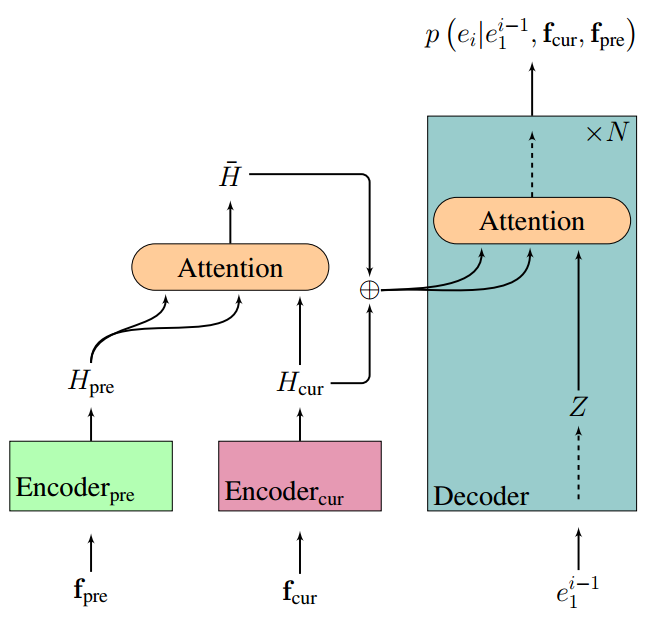
\includegraphics[width=0.90\linewidth]{Images/models_outide_decoder}
				\label{fig:modelsoutidedecoder}
			\end{figure}
		\end{column}%
	\end{columns} 
\end{frame}

\begin{frame}{Separate Encoding Approaches}
	Once the encoding of the current and the context sentences has been carried out, they can be integrated in different ways:
	\begin{columns}[T] % align columns
		\begin{column}{.50\textwidth}
			\begin{itemize}
				\item \textbf{Outside} the decoder.
					\begin{itemize}
						\item (+) symbol represents a gate, a sum or a concatenation.
					\end{itemize}
				\item \textbf{Inside} the decoder, \textbf{sequentially}. 
			\end{itemize}
		\end{column}%
		\hfill%
		\begin{column}{.50\textwidth}
			\begin{figure}
				\centering
				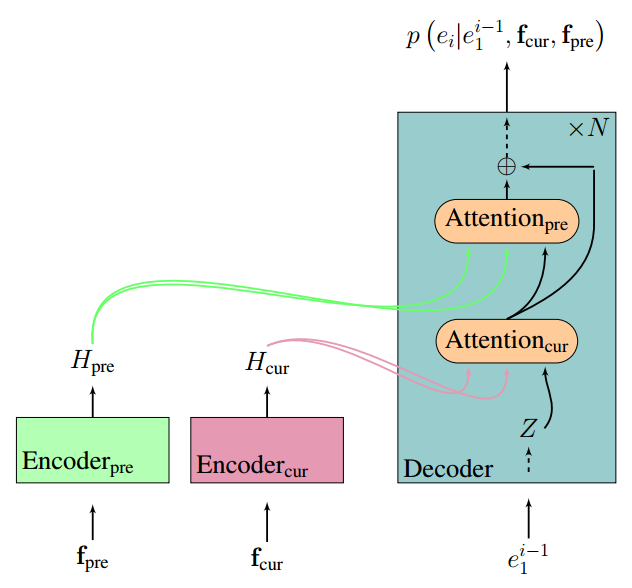
\includegraphics[width=0.90\linewidth]{Images/models_inside_decoder_sequential}
				\label{fig:modelsoutidedecoder}
			\end{figure}
		\end{column}%
	\end{columns} 
\end{frame}

\begin{frame}{Separate Encoding Approaches}
	Once the encoding of the current and the context sentences has been carried out, they can be integrated in different ways:
	\begin{columns}[T] % align columns
		\begin{column}{.50\textwidth}
			\begin{itemize}
				\item \textbf{Outside} the decoder.
					\begin{itemize}
						\item (+) symbol represents a gate, a sum or a concatenation.
					\end{itemize}
				\item \textbf{Inside} the decoder, \textbf{sequentially}.
				\item \textbf{Inside} the decoder, \textbf{in parallel}. 
			\end{itemize}
		\end{column}%
		\hfill%
		\begin{column}{.50\textwidth}
			\begin{figure}
				\centering
				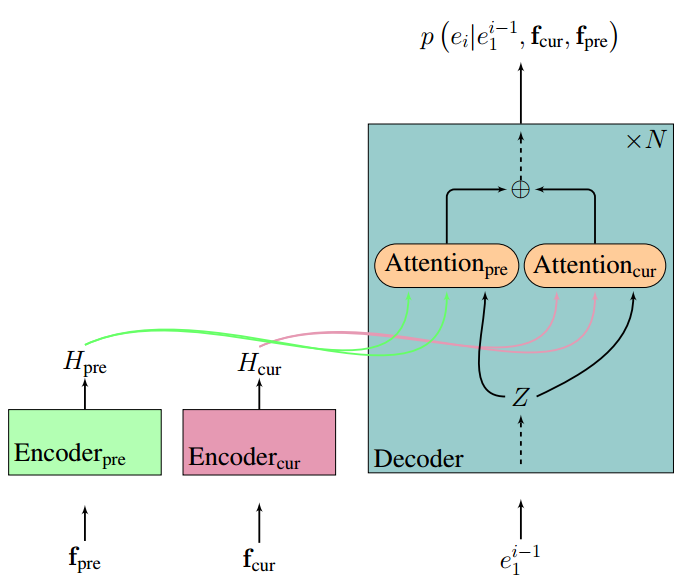
\includegraphics[width=0.90\linewidth]{Images/models_inside_decoder_parallel}
				\label{fig:modelsoutidedecoder}
			\end{figure}
		\end{column}%
	\end{columns} 
\end{frame}

\begin{frame}{Separate Encoding Approaches}
	\textbf{Architecture}\\
	The encoder-decoder architectures depicted above can be both RNN-based (until 2017) or Transfomer-based (after 2017), as for any approach to DLNMT. However, often some modifications are applied. For example:
	\begin{itemize} 
		\item In the case of RNN-based architectures, integration inside the decoder can be undertaken without attention by simply concatenating context representations to the cell state of the deocdrr's RNN \cite{wang_exploiting_2017}.
		\item  beside contextual representation of words, the context encoder can also higher level representations such as sentence or document representations. This representations can also be attended by the decoder \cite{miculicich_document-level_2018, maruf_selective_2019} or added to the word-representations \cite{tan_hierarchical_2019}.
		\item Parallel integration inside the decoder can also happen within a single multi-head attention that takes as values and queries the concatenations of the current and context sentence representations \cite{voita_when_2019}
	\end{itemize}
\end{frame}

\begin{frame}{Separate Encoding Approaches}
	\textbf{Including target-side context}\\
	Despite some have considered including past target-side context harmful because of the \textit{error propagation} problem \cite{zhang_improving_2018}, most recent works have showed it to be of utmost importance for making the most out of context. Past works have successfully included target-side context information in different ways:
	\begin{itemize}
		\item Translating past sentences (usually 1) along with the current one, and then discarding them, as in concatenation approaches \cite{bawden_evaluating_2018}.
		\item By making the decoder attend the target-side hidden representations or embeddings of previously decoded sentences \cite{miculicich_document-level_2018,voita_when_2019,maruf_selective_2019,zheng_toward_2020}.
	\end{itemize}
\end{frame}

\begin{frame}{Multi-Encoder}\label{slide:separateencoding}
	\begin{table}
		\begin{tabular}{ *{5}{c|} c }

			\thead{Reference}
			& \thead{Context}
					& \thead{Two-Pass\\ Approach}
						& \thead{Outside\\ Integr.}
							& \thead{Inside\\ Integr.}
								& \thead{Lang.\\ Pair}
									 \\
			\hline\hline
			\cite{wang_exploiting_2017}&s:-3 &&aut...&...aut&Zh$\to$En\\
			\hline
			\cite{voita_context-aware_2018}&s:-1&&yes&&En$\to$Ru\\
			\hline
			\cite{zhang_improving_2018}&s:-2&&yes&sequential&Zh$\to$En\\
			\hline
			\cite{miculicich_document-level_2018}&s:-3; t:-3&&yes&&Zh/Es$\to$En\\
			\hline
			\cite{maruf_selective_2019}&s:all; t:all&optional&yes&&En$\to$De\\
			\hline
			\cite{zheng_toward_2020}&s:all; t:all&yes&yes&&Zh/En$\to$En/De\\
			\hline
			\cite{jean_does_2017}&s:-1&&&parallel&En$\to$De/Fr\\
			\hline
			\cite{bawden_evaluating_2018}&s:-1; t:-1&&&parallel&En$\to$Fr\\
			\hline
			\cite{fu_reference_2019}&s:all&yes&&parallel&En/Zh$\to$De/En\\
			\hline
			\cite{tan_hierarchical_2019}&s:all&yes&&parallel&Zh/De$\to$En\\
			\hline
			\cite{voita_when_2019}&s:-3; t:-3&yes&&parallel*&En$\to$Ru\\
			\hline
		\end{tabular}
	\end{table}
\end{frame}

%%%%%%%%%%%%%%%%%%%%%%%%%%%%%%%%%%%%%%%%%%%%%%%%%%%%%%%%%%%%%%%%%%%%%%%%%
\subsection{Caches}

\begin{frame}{Caches}
\begin{itemize}
	\item \cite{maruf_document_2018} \textbf{Two-pass approach \textcolor{red}{(not training! to explain...)}. All context (source and target). Fr/De/Et$\to$En. Decoder without attention (integration in the RNN gates).} First pass for sentence representations (filling the memories), second pass for integrating current sentence representation with information stocked into memories (via coarse attention). \textcolor{red}{extention: attention to target memory!}
	\item \cite{zheng_learning_2018} borrow the decoder architecture from the TransformerXL \cite{dai_transformer-xl_2019}. This is very similar to the Transformer's decoder, but every time it translates a sentence it keeps its hidden representations into memory so that it can attend to them while decoding the following sentence. This mechanism creates a recurrence that enables past target-side information to be remembered.
\end{itemize}
\end{frame}

%%%%%%%%%%%%%%%%%%%%%%%%%%%%%%%%%%%%%%%%%%%%%%%%%%%%%%%%%%%%%%%%%%%%%%%%%
\subsection{Others}

\begin{frame}{Others}
\textbf{discourse-related information}
	\begin{itemize}
		\item \cite{ohtani_context-aware_2019} concatenates multiple inputs (past and future), up to -7+3, Bi-LSTM, En->Jap. Add coreference information to the input and modify lstm to merge into its hidden state the antecedent or descendant's hidden states.
		\item \cite{stojanovski_coreference_2018} see survey
		\item \cite{rios_gonzales_improving_2017} see survey
	\end{itemize}
\end{frame}

\begin{frame}{Others}
\textbf{using monolingual corpora}
	\begin{itemize}
		\item \cite{martinez_garcia_context-aware_2019} generate translation by integrating the scores output by Semantic Space Language Model and a NMT model, following the shallow fusion strategy \cite{gulcehre_using_2015}.
		\item \cite{sugiyama_data_2019} augment dl parallel data by backtranslating BookCorpus (En->Ja). Then finds that the synthetic dl parallel corpus improves training of a DLNMT Transformer with concatenation of the inputs. Parallel corpus: IWSLT2017, Ja/Fr->En. Improvements are visible in both terms of BLUE but also discourse phenomena.
		\item \cite{jean_context-aware_2019} inputing context sentences with different strategies.
		\item \cite{li_pretrained_2019} pre-trained BERT for initializing the encoder
		\item \cite{voita_context-aware_2019} Automatic Post Editing from sentence level to context level.
	\end{itemize}
\end{frame}

\begin{frame}{Others}
\textbf{dlnmt as learning problem}
	\begin{itemize}
		\item \cite{jean_context-aware_2019} 
	\end{itemize}
\end{frame}

%%%%%%%%%%%%%%%%%%%%%%%%%%%%%%%%%%%%%%%%%%%%%%%%%%%%%%%%%%%%%%%%%%%%%%%%%

\begin{frame}{Positional embedding schemas}
		\begin{enumerate}
			\item positional encoding \cite{vaswani_attention_2017}
			\item sentence distance embedding \cite{voita_when_2019}
			\item inverse embedding and shit \cite{maruf_contextual_2018}
			\item segment embedding \cite{zheng_toward_2020}
		\end{enumerate}
\end{frame}

\begin{frame}{Notes}
	\begin{enumerate}
		\item two-step training what is. E.g. \cite{zhang_improving_2018, miculicich_document-level_2018}. Explain that DL training corpus is small! possible future direction...
		\item using reference translations as target context during training have been proven useful but only to a certain extent. Better to mix reference with candidate outputs \cite{voita_when_2019}
	\end{enumerate}
\end{frame}

%%%%%%%%%%%%%%%%%%%%%%%%%%%%%%%%%%%%%%%%%%%%%%%%%%%%%%%%%%%%%%%%%%%%%%%%%
\subsection{Remarks and conclusions}

\begin{frame}{Remarks and conclusions}
	\textbf{Possible Future Research Directions}
	\begin{itemize}
		\item build a large DL corpus for training systems;
		\item design models exploiting full context;
		\item design models performing  good for single-sentence translation \cite{zheng_toward_2020}
		\item design post-processing models that are lightweight and can be trained on little data \cite{kim_when_2019}. Nonetheless, beware that While this kind of approach is easy to deploy, the two-stage generation process may result in error accumulation.
	\end{itemize}
\end{frame}

%\begin{frame}{Regret}
%
%	\begin{columns}
%	\begin{column}{0.6\textwidth}
%	 \onslide<+->\begin{block}{Sub-linear Regret}
%	\begin{enumerate}
%			\item<+-|alert@+> for any linear function $f(T)$, for sufficiently large input $T$, $Regret(T)$ grows slower than $f(T)$.
%			\item<+-|alert@+> Alternatively, $\lim_{T\to\infty}Regret(T)/T=0$
%		\end{enumerate}
%	\end{block}
%	\end{column}
%
%	\begin{column}{0.4\textwidth}
%		\centering
%		\includegraphics<+->[width=1\textwidth]{Images/mabomber}
%	\end{column}
%	\end{columns}
%\end{frame}


%\begin{frame}{A useful formulation}
%
%	\begin{columns}
%	\begin{column}{0.4\textwidth}
%	  \begin{center}
%	     \includegraphics<+->[width=1\textwidth]{Images/mabomber}
%	  \end{center}
%%	    \quad Multi \hspace{0.80cm} Armed \hspace{0.70cm} Bandits
%	\end{column}
%
%	\begin{column}{0.6\textwidth}
%	\begin{block}{Multi Armed Bandits}
%	    \begin{itemize}
%	    \item<+-|alert@+> Simpler framework;
%	    \item<+-|alert@+> Share the exploration-exploitation tradeoff;
%	    \item<+-|alert@+> Ample literature available.
%	    \end{itemize}
%	 \end{block}
%	 
%	 \onslide<+->{	
%	\begin{block}{Regret}
%	 $Regret(T)=\mathcal{O}(\sqrt T)\to$ regret is \textbf{sub-linear}.
%	\end{block}
%	}
%	
%%	\onslide<+->{	
%%	\begin{block}{Desideratum}
%%	 \textbf{sub-linear} $Regret(T)\Leftrightarrow \lim_{T\to\infty}Regret(T)/T=0$
%%	 \\~\\
%%	 E.g. $Regret(T)=\mathcal{O}(\log T)$
%%	\end{block}
%%	}
%%	
%	\end{column}
%	\end{columns}
%\end{frame}


%	\onslide<2->{
%	\textbf{Rewards}: portfolio log-return with transaction costs
%		\begin{equation*}
%			R_{t+1} = \log \left\{ 1 + \sum^{I}_{i=0} \left[ 
%				\tikz[baseline]{
%		        	\node[anchor=base] (t1) {$a_t^i X_{t+1}^i$};
%		        } - 
%		        \tikz[baseline]{
%		        	\node[anchor=base] (t2) {$\delta_i \left| a_t^i - \widetilde{a}_t^i \right|$};
%		       	} -
%		       	\tikz[baseline]{
%		       		\node[anchor=base] (t3) {$\delta_s {(a_t^i)}^-$};
%		       	} \right] -
%		       	\tikz[baseline]{
%		       		\node[anchor=base] (t4) {$\delta_f \mathbf{1}_{{a}_t \neq \tilde{{a}}_{t-1}}$};
%		       	} \right\}	 	
%		 \end{equation*}
%	}
%	
%	\onslide<7->{
%	\textbf{Actions}: Portfolio weights
%		\begin{equation*}
%			\{a_t^i\}_{i=0}^I \;\;\; \text{s.t.}\;\;\; \sum^{I}_{i=0} a_t^i = 1 \;\;\;\;\; \forall t \in \{0, 1, 2, \ldots\}
%		\end{equation*}
%	}
%
%	\onslide<8->{
%	\textbf{States}: assets past returns and current allocation
%		\begin{equation*}
%			S_t = \{X, X_t, X_{t-1}, \ldots, X_{t-P}, \tilde{a}_t\}
%		\end{equation*}
%	}
%	
%	\onslide<3|handout:0>{
%		\begin{tikzpicture}[overlay]
%				\node[draw=SteelBlue, circle, line width=3pt, minimum size=2cm] at (t1) {};
%		\end{tikzpicture}
%	}
%	
%	\onslide<4|handout:0>{
%		\begin{tikzpicture}[overlay]
%				\node[draw=SteelBlue, circle, line width=3pt, minimum size=2cm] at (t2) {};
%		\end{tikzpicture}
%	}
%		
%	\onslide<5|handout:0>{
%		\begin{tikzpicture}[overlay]
%				\node[draw=SteelBlue, circle, line width=3pt, minimum size=2cm] at (t3) {};
%		\end{tikzpicture}
%	}
%			
%	\onslide<6|handout:0>{
%		\begin{tikzpicture}[overlay]
%				\node[draw=SteelBlue, circle, line width=3pt, minimum size=2cm] at (t4) (g) {};
%		\end{tikzpicture}
%	}
%\end{frame}
%
%\begin{frame}[c]{Synthetic Asset: Convergence}
%\begin{figure}[t!]
%	\centering
%	\includegraphics[height=5cm,width=0.8\textwidth]{Images/6_0_single_synthetic_neutral_convergence}
%\end{figure}
%\end{frame}
%
%
%\begin{frame}[c]{Synthetic Asset: Backtest Performance}
%\begin{figure}[t]
%	\centering
%	\includegraphics[height=6cm,width=0.8\textwidth]{Images/6_1_single_synthetic_neutral_performance}
%\end{figure}
%\end{frame}
%
%\begin{frame}[c]{Synthetic Asset: Impact of Transaction Costs}
%\begin{figure}[t!]
%	\centering
%	\includegraphics[height=3cm,width=0.8\textwidth]{Images/6_2_impact_transaction_costs}
%\end{figure}
%\begin{figure}[t!]
%	\centering
%	\includegraphics[height=3cm,width=0.8\textwidth]{Images/6_3_impact_short_selling_fees}
%\end{figure}
%\end{frame}
%
%\begin{frame}{Not So Fast}
%
%	\onslide<1->{
%	\begin{columns}
%	\begin{column}{0.6\textwidth}
%	   \begin{alertblock}{Insuccess on Historical Data}
%	   Successfully applying these RL algorithms to historical data is much more challenging
%	   \begin{enumerate}
%	   		\item Fail to converge
%	   		\item The strategies learned are not profitable
%	   \end{enumerate}
%	   \end{alertblock}
%	\end{column}
%	\begin{column}{0.4\textwidth}
%	    \begin{center}
%	     \includegraphics[width=1\textwidth]{Images/8_9_single_hist_neutral_performance}
%	     \end{center}
%	\end{column}
%	\end{columns}
%	}
%	
%	\onslide<2->{	
%	\begin{block}{Possible Explanations}
%		\begin{enumerate}
%			\item<2-> \textbf{Low signal-to-noise ratio}: extremely difficult to find tradable patterns in markets
%			\item<3-> \textbf{Quality of data}: unlikely to find patterns in daily prices of liquid stocks
%			\item<4-> \textbf{Weak features}: parametric policy must be powerful enough to capture the signal
%			\item<5-> \textbf{Non-stationarity of financial time-series}: a signal needs to be persistent
%		\end{enumerate}
%	\end{block}
%	}

